%!TEX TS-program = xelatex

% Этот шаблон документа разработан в 2014 году
% Данилом Фёдоровых (danil@fedorovykh.ru) 
% для использования в курсе 
% <<Документы и презентации в \LaTeX>>, записанном НИУ ВШЭ
% для Coursera.org: http://coursera.org/course/latex .
% Исходная версия шаблона --- 
% https://www.writelatex.com/coursera/latex/5.2.2

\documentclass[a4paper,12pt]{article}

%%% Работа с русским языком
\usepackage[english,russian]{babel}   %% загружает пакет многоязыковой вёрстки
\usepackage{fontspec}      %% подготавливает загрузку шрифтов Open Type, True Type и др.
\defaultfontfeatures{Ligatures={TeX},Renderer=Basic}  %% свойства шрифтов по умолчанию
\setmainfont[Ligatures={TeX,Historic}]{Times New Roman} %% задаёт основной шрифт документа
\setsansfont{Comic Sans MS}                    %% задаёт шрифт без засечек
\setmonofont{Courier New}
\usepackage{indentfirst}
\frenchspacing

\renewcommand{\epsilon}{\ensuremath{\varepsilon}}
\renewcommand{\phi}{\ensuremath{\varphi}}
\renewcommand{\kappa}{\ensuremath{\varkappa}}
\renewcommand{\le}{\ensuremath{\leqslant}}
\renewcommand{\leq}{\ensuremath{\leqslant}}
\renewcommand{\ge}{\ensuremath{\geqslant}}
\renewcommand{\geq}{\ensuremath{\geqslant}}
\renewcommand{\emptyset}{\varnothing}

%%% Дополнительная работа с математикой
\usepackage{amsmath,amsfonts,amssymb,amsthm,mathtools} % AMS
\usepackage{icomma} % "Умная" запятая: $0,2$ --- число, $0, 2$ --- перечисление

%% Номера формул
%\mathtoolsset{showonlyrefs=true} % Показывать номера только у тех формул, на которые есть \eqref{} в тексте.
%\usepackage{leqno} % Нумерация формул слева

%% Свои команды
\DeclareMathOperator{\sgn}{\mathop{sgn}}

%% Перенос знаков в формулах (по Львовскому)
\newcommand*{\hm}[1]{#1\nobreak\discretionary{}
	{\hbox{$\mathsurround=0pt #1$}}{}}

%%% Работа с картинками
\usepackage{graphicx}  % Для вставки рисунков
\graphicspath{{images/}{images2/}}  % папки с картинками
\setlength\fboxsep{3pt} % Отступ рамки \fbox{} от рисунка
\setlength\fboxrule{1pt} % Толщина линий рамки \fbox{}
\usepackage{wrapfig} % Обтекание рисунков текстом

%%% Работа с таблицами
\usepackage{array,tabularx,tabulary,booktabs} % Дополнительная работа с таблицами
\usepackage{longtable}  % Длинные таблицы
\usepackage{multirow} % Слияние строк в таблице

%%% Теоремы
\theoremstyle{plain} % Это стиль по умолчанию, его можно не переопределять.
\newtheorem{theorem}{Теорема}[section]
\newtheorem{proposition}[theorem]{Утверждение}

\theoremstyle{definition} % "Определение"
\newtheorem{corollary}{Следствие}[theorem]
\newtheorem{problem}{Задача}[section]

\theoremstyle{remark} % "Примечание"
\newtheorem*{nonum}{Решение}

%%% Программирование
\usepackage{etoolbox} % логические операторы


%%% Страница
\usepackage{extsizes} % Возможность сделать 14-й шрифт
\usepackage{geometry} % Простой способ задавать поля
\geometry{top=5mm}
\geometry{bottom=15mm}
\geometry{left=5mm}
\geometry{right=5mm}
%
%\usepackage{fancyhdr} % Колонтитулы
% 	\pagestyle{fancy}
%\renewcommand{\headrulewidth}{0pt}  % Толщина линейки, отчеркивающей верхний колонтитул
% 	\lfoot{Нижний левый}
% 	\rfoot{Нижний правый}
% 	\rhead{Верхний правый}
% 	\chead{Верхний в центре}
% 	\lhead{Верхний левый}
%	\cfoot{Нижний в центре} % По умолчанию здесь номер страницы

\usepackage{setspace} % Интерлиньяж
%\onehalfspacing % Интерлиньяж 1.5
%\doublespacing % Интерлиньяж 2
%\singlespacing % Интерлиньяж 1

\usepackage{lastpage} % Узнать, сколько всего страниц в документе.

\usepackage{soul} % Модификаторы начертания

\usepackage{hyperref}
\usepackage[usenames,dvipsnames,svgnames,table,rgb]{xcolor}
\hypersetup{				% Гиперссылки
	unicode=true,           % русские буквы в раздела PDF
	pdftitle={Заголовок},   % Заголовок
	pdfauthor={Автор},      % Автор
	pdfsubject={Тема},      % Тема
	pdfcreator={Создатель}, % Создатель
	pdfproducer={Производитель}, % Производитель
	pdfkeywords={keyword1} {key2} {key3}, % Ключевые слова
	colorlinks=true,       	% false: ссылки в рамках; true: цветные ссылки
	linkcolor=red,          % внутренние ссылки
	citecolor=black,        % на библиографию
	filecolor=magenta,      % на файлы
	urlcolor=cyan           % на URL
}

\usepackage{csquotes} % Еще инструменты для ссылок

%\usepackage[style=authoryear,maxcitenames=2,backend=biber,sorting=nty]{biblatex}

\usepackage{multicol} % Несколько колонок

\usepackage{tikz} % Работа с графикой
\usepackage{pgfplots}
\usepackage{pgfplotstable}

\author{Батарин Егор}
\title{Амплитудная дифракционная решетка.}
\date{\today}

\begin{document} % конец преамбулы, начало документа
	
	\maketitle
	
	\begin{abstract}
		
		Знакомство с работой и настройка гониометра Г5, определение спектральных характеристик амлитудной решетки.
		
	\end{abstract}
	

\section{Теория}

\subsection{Общие понятия}
Оптические приборы, в которых осуществялется физическое разложение электромагнитного излучения намонохроматические составляющие, называются спектральными. По характеру распределения интенсивности вспектральном разложении спектры могут быть разделены на линейчатые и непрерывные. \par 
Принципиальная установка изображена на рис.\ref{p1}. Свет от источника S попадает на экран с щелью. Коллиматор формирует близкие к параллельному пучок лучей. После, свет попадает надиспергирующий элемент.Наблюдейние производится через трубу, установленну на $\infty$


\begin{figure}[h!]
	\begin{center}
		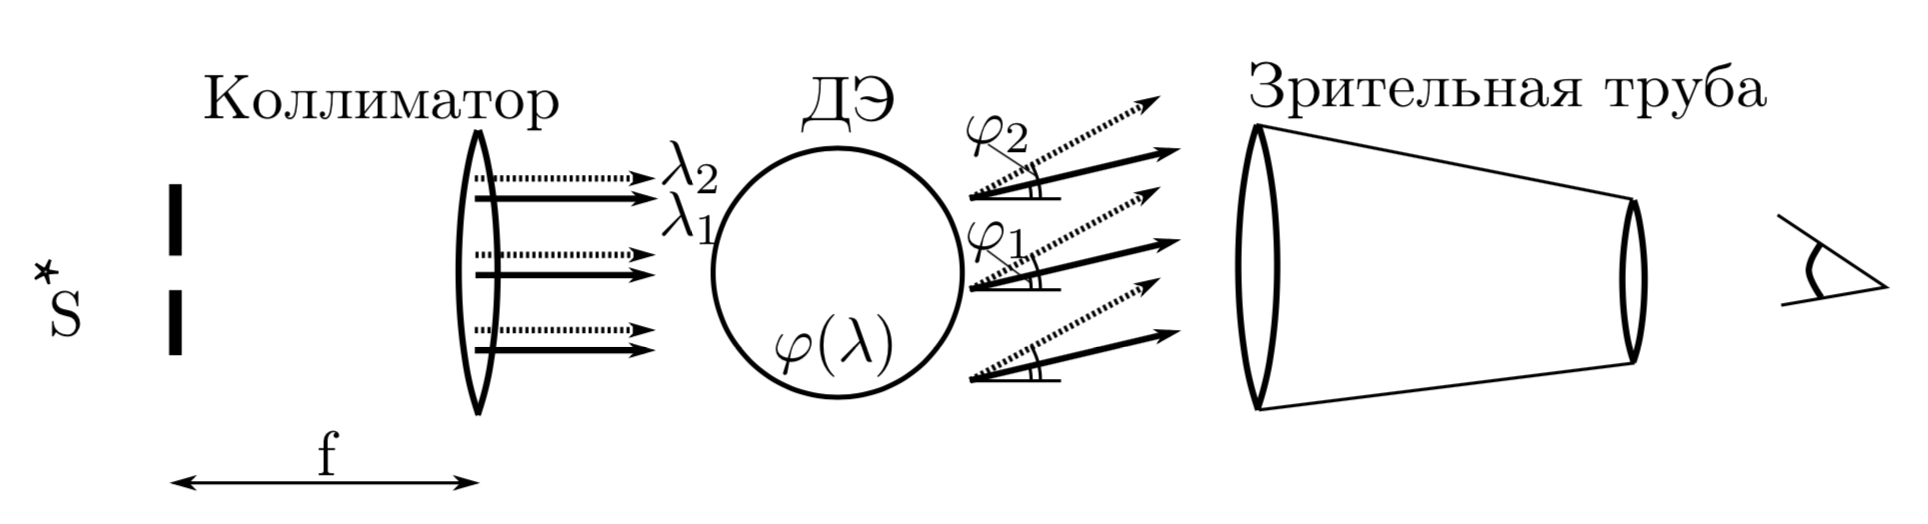
\includegraphics[scale = 0.5]{p1.png}
		\caption{Схема прибора: источник-коллиматор – диспергирующий элемент – зрительная труба}
		\label{p1}
	\end{center}
\end{figure}

Каждой монохроматической компоненте с $\lambda$ соответствует один или несколько углов $\varphi(\lambda)$ на выходе изприбора, в направлении которых интенсивность прибора максимальна. При известной зависимости $\varphi(\lambda)$ поизмеряемому углу поворота $\varphi$ зрительной трубы можно определить длинну волны спектральной линии. \par 
Наиболее важными характеристиками спектральных приборов являютсяугловая дисперсия, разрешающая способность и дисперсионная область.


\subsection{Амплитудная дифракционная решетка}

Амплитадная решетка представляет собой N паралельных щелей (рис.2), период решетки равен d, ширинаштриха - b. Наблюдение ведем на бесконечности (дифракция Фраунгофера). Амплитуда и интенсивность поля
световой волны определяются углом $\varphi$. Полагаем, что амплитуда падающих лучей одинкова. Интенсивность дифрагированного света максимальная для углов $\varphi_m$, при которых волны, приходящие в точку наблюдения оказываются в фазе:

\begin{equation}
d \sin{\varphi_m} = m\lambda
\end{equation}

\begin{figure}[h!]
	\begin{center}
		\begin{minipage}[h]{0.3\linewidth}
			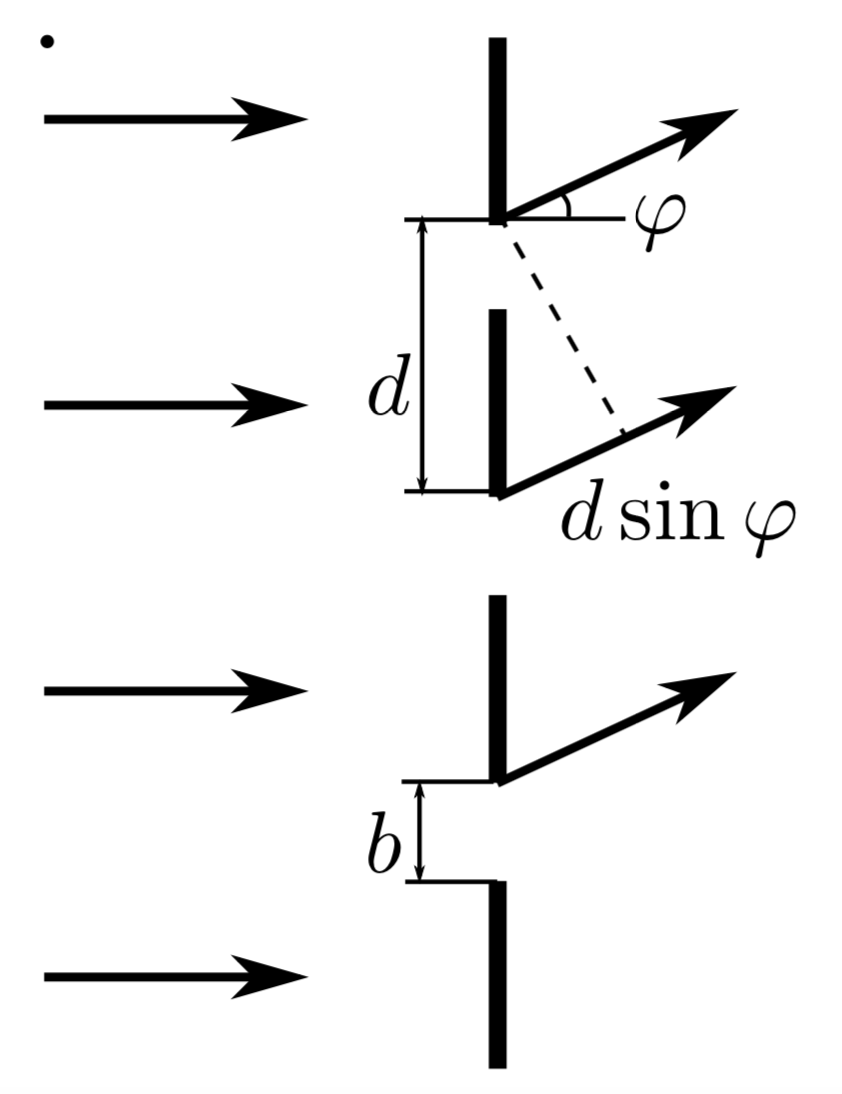
\includegraphics[width=1\linewidth]{p2.png}
			\caption{Дифракция световой волны на амплитудной решетке} 
			\label{p2}
		\end{minipage}
		\hfill 
		\begin{minipage}[h]{0.45\linewidth}
			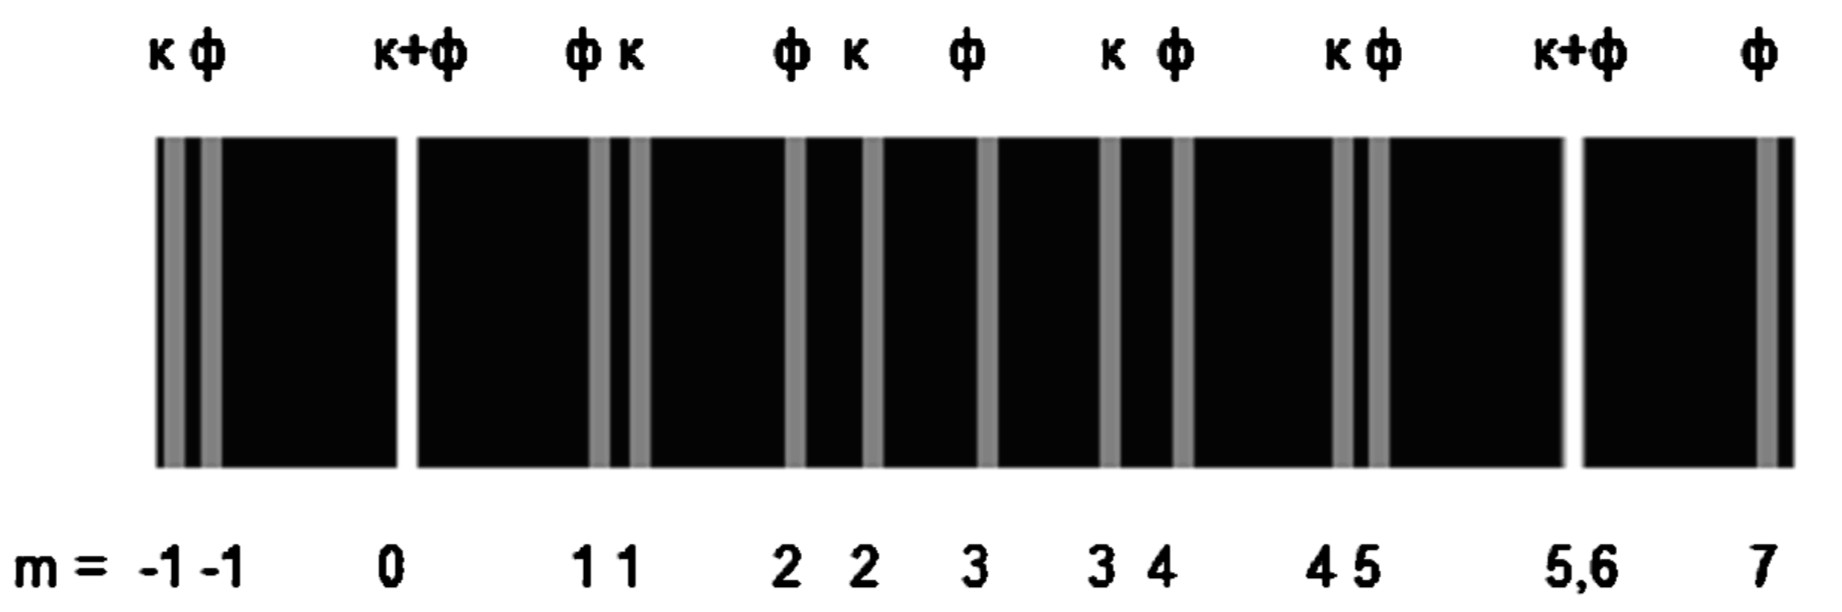
\includegraphics[width=1\linewidth]{p3.png}
			\caption{Изображение спектра двух линий}
			\label{p3}
		\end{minipage}
	\end{center}
\end{figure}

Рассмотрим пример с двумя спектральными линиями красной и фиолетовой $(\lambda_{red}> \lambda_{purp})$ рис.3. Для малых углов дифракции угловое расстояние между порядками $\varphi_{m+1} - \varphi \approx \lambda /d$ пропорционально длине волны, поэтому фиолетовые линии следуют чаще чем красные. При $m = 5$ для красной и $m = 6$ для фиолетовой они совпадут. \par 

Некоторые формулы:

\begin{itemize}
	\item Разрешающая способность характеризует возможность прибора различать две близкие спектральные линии с длинами волн $\lambda$ и $\lambda + \delta \lambda$.
	\begin{equation}
	R = \frac{\lambda}{\delta \lambda}
	\end{equation}
	
	\item Угловая дисперсия - производная зависимости угла отклонения $\varphi(\lambda)$ волны диспергирующим элементом по $\lambda$. По величине угловой дисперсии можно определить угловое расстояние между двумя близкими спектральными линиями: $\delta \varphi \approx D \delta \lambda$:
	
	\begin{equation}
	D = \frac{d \varphi}{d \lambda} = \frac{m}{d \cdot \cos{\varphi_m}} = \frac{m}{\sqrt{d^2 - m^2 \lambda^2}}
	\end{equation}
	
	\item Угловое расстояние между линиями определяется:
	\begin{equation}
	\Delta \varphi \approx D \delta \lambda
	\end{equation}
	
	\item Полуширина линии:
	\begin{equation}
	\delta \varphi = \frac{\lambda}{Nd \cos{\varphi_m}}
	\end{equation}
	
	\item Дисперсионная область – предельная ширина спектального интервала $\Delta \lambda$ прибора, для которой дифракционные максимумы соседних порядков не перекрываются. Она определяет диапазон длин волн, при которых прибор может быть использован для анализа спектра.
	
\end{itemize}


\section{Ход работы}

\begin{enumerate}
	\item Настроим гониометр
	\item Установим решетку, откалибруем наклон столика.
	\item Подберем ширину входной щели так, чтобы ширина желктого дуплета была чуть больше промежутка между линиями двойного штриха окуляра.
	\item Измерим угловые координаты спектральных линий ртути в $\pm 1$ порядке и занесем в таблицу \ref{t1}
	
	\begin{table}[h!]
		\begin{center}
			\begin{tabular}{|c|c|c|c|}
				\hline
				Цвет & Угол & Длина волны, $\lambda, \; нм$ & Порядок \\ \hline 
				Синий & 192 $^{\circ}$ 33'&435.80& 1\\ \hline
				Зеленый & 194 $^{\circ}$ 10' & 546.07 & 1 \\\hline
				Желтый & 196 $^{\circ}$ 41' &576.96 & 1 \\ \hline
				Красный & 197 $^{\circ}$ 35' & 623.40 & 1\\ \hline
				Синий & 167 $^{\circ}$ 24' & 435.80 & -1 \\ \hline 
				Зеленый & 164 $^{\circ}$ 09' & 546.07 & -1 \\\hline
				Желтый & 163 $^{\circ}$ 12' &576.96 & -1 \\ \hline
				Красный & 161 $^{\circ}$ 50' & 623.40 & -1\\ \hline
				
			\end{tabular}
			\caption{}
			\label{t1}
		\end{center}
	\end{table}
	
	\item Построим зависимость $\sin{\varphi_m}$ от длины волны:
	\begin{figure}[h!]
		\begin{center}
			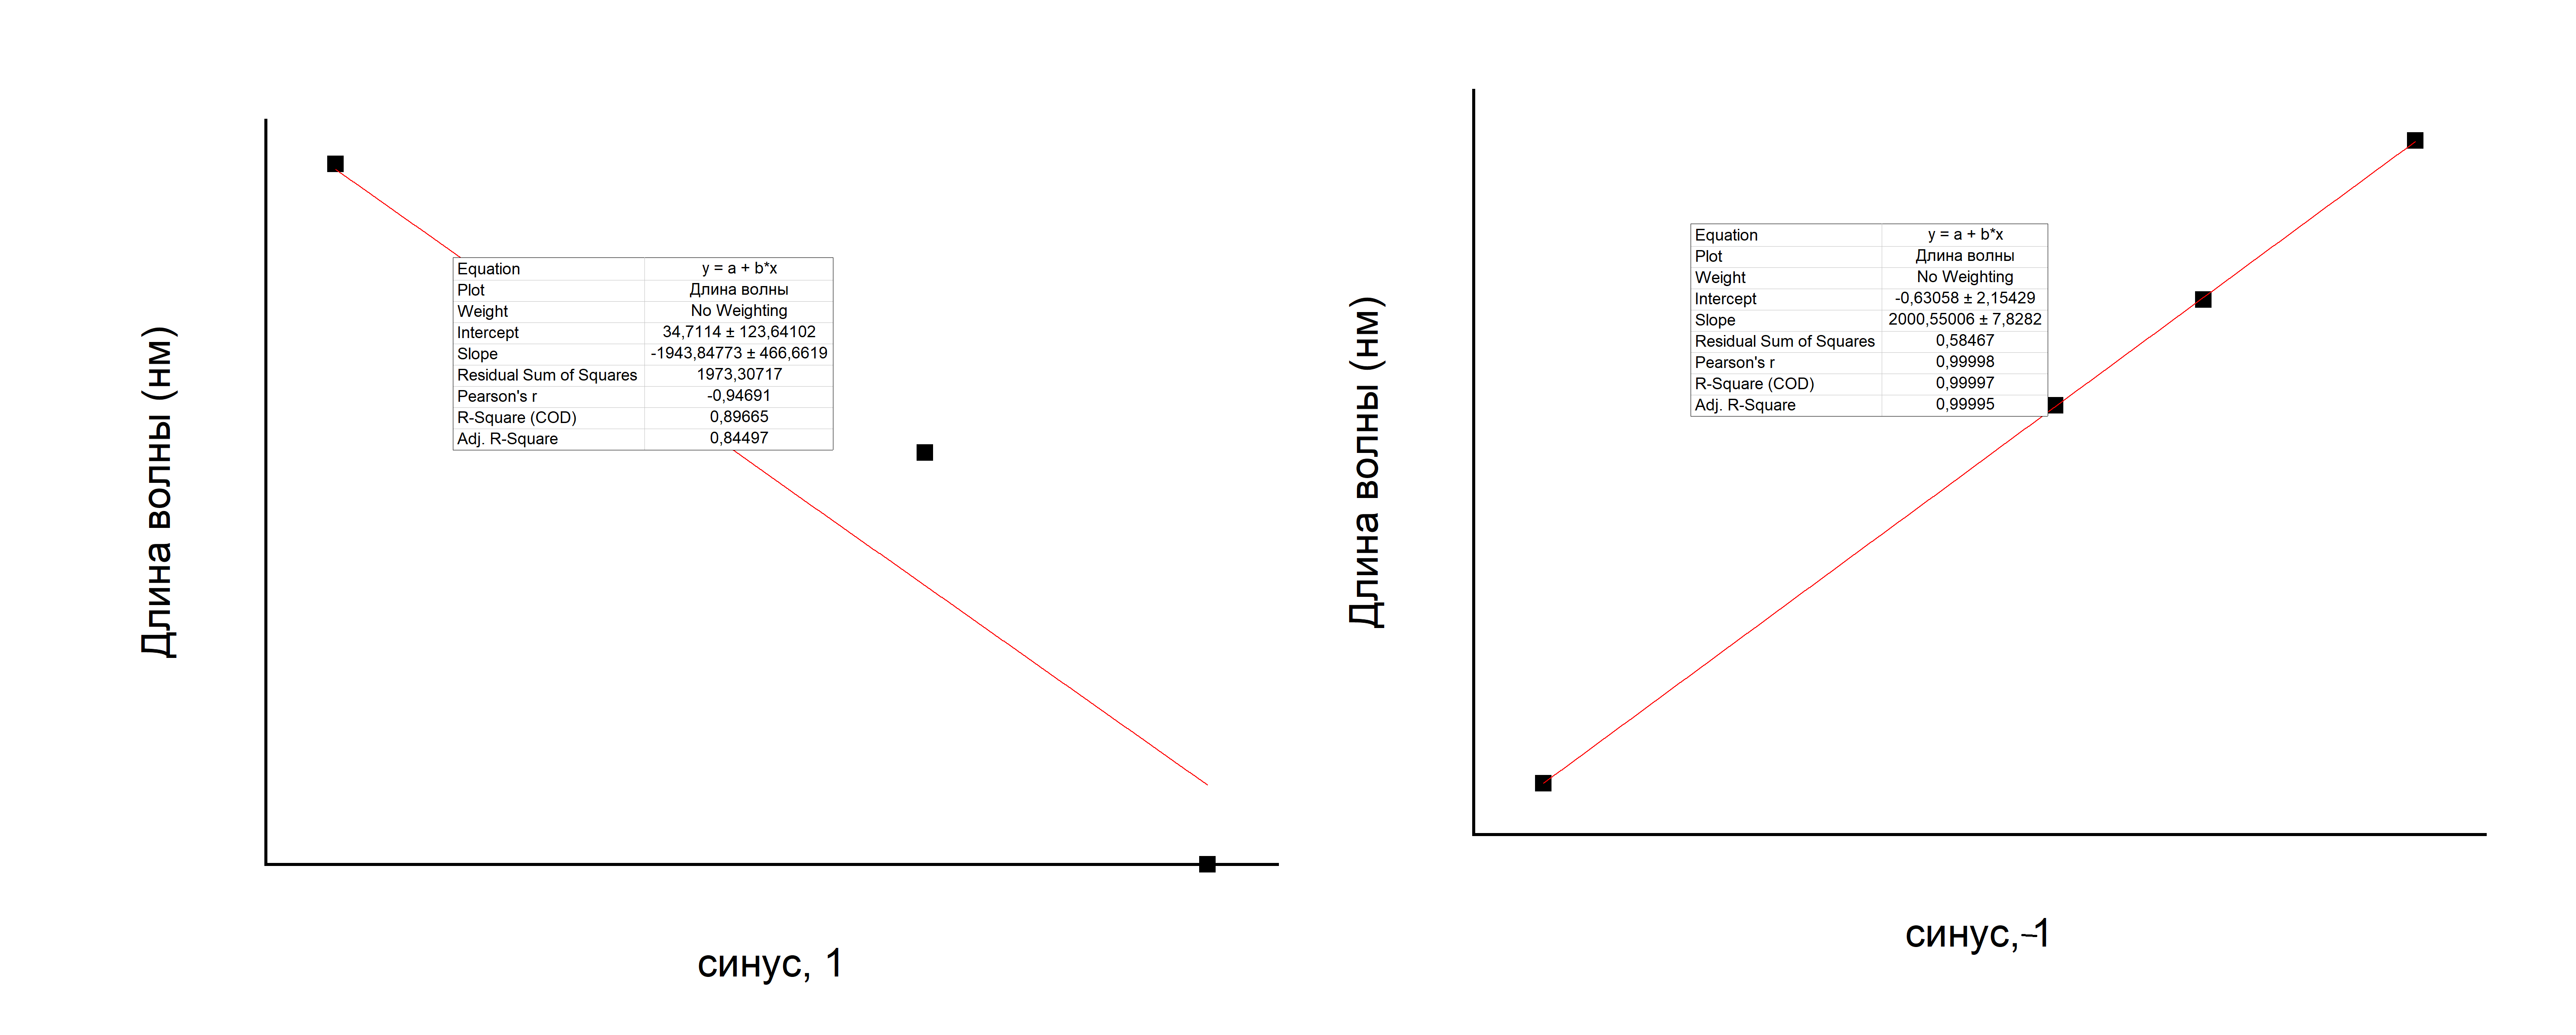
\includegraphics[scale = 0.3]{228.png}
			\caption{Зависимость $\lambda(\sin \phi_m)$}
			\label{p1}
		\end{center}
	\end{figure}

	\item Найдем период дифракционной решетки с помощью формулы $d \sin{\varphi_m} = m\lambda$ и МНК:
	$d= 1,98 \pm 0,35 \text{мкм}$
	\item Для оценки угловой дисперсии решетки измерим угловые координаты линий желтого дуплета на всех видимых порядках, результат занесем в таблицу \ref{t2}.
	
	\begin{table}[h!]
		\begin{center}
			\begin{tabular}{|c|c|c|c|c|c|c|c|c|}
				\hline
				Порядок&-1&-1&1&1&2&2&-2&-2 \\ \hline 
				$\lambda, \;nm$&576.96&579.09&576.96&579.07&579.96&576.09&576.96&579.07 \\ \hline
				$\Delta \lambda, \; nm$& -2.13&&-2.11&&-2.13&&-2.11& \\ \hline
				$\varphi_m,^{\circ}$& 196.68& 196.75 &163.17 & 163.24& 144.60& 144.64& 215.09& 215.15 \\ \hline 
				$\Delta \varphi_m,^{\circ}$& -0.0641&& -0.066 && -0.036 && -0.036 & \\ \hline 
				D, рад/мкм& 0,31635&0,31645-&0,31658&-0,31647&-0,74348&-0,74314&0,74076&0,74109 \\ \hline
			\end{tabular}
			\caption{}
			\label{t2}
		\end{center}
	\end{table}
	
	\item Рассчитаем по линиям желтого дуплета угловую дисперсию в спектрах разного порядка по формуле $D(\lambda) = \frac{d \varphi}{d \lambda}$, результат занесем в таблицу \ref{t2}.
	Построим график зависимости угловой дисперсии от порядка спектра и сравним с рассчитанной по формуле $D = \frac{d \varphi}{d \lambda} = \frac{m}{d \cdot \cos{\varphi_m}} = \frac{m}{\sqrt{d^2 - m^2 \lambda^2}}$.
	
	\begin{figure}[h!]
		\begin{center}
			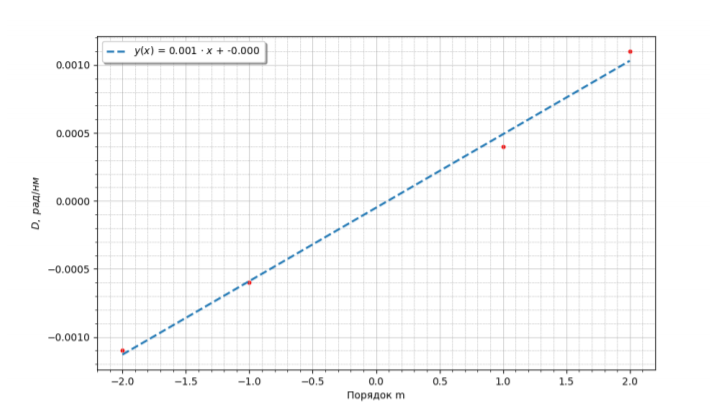
\includegraphics[scale = 1]{5.png}
			\caption{Зависимость угловой дисперсии от порядка}
			\label{p1}
		\end{center}
	\end{figure}
	
	\item Оценим разрешимый спеткральный интервал $\delta \lambda$, результат занесем в таблицу \ref{t2}. По формуле $\Delta \varphi \approx D \delta \lambda = \frac{m}{d \cos{\varphi_m}} \delta \lambda$ определим угловую ширину желтой линии. 
	\item По формуле $R = \frac{ \lambda}{\delta \lambda} = 978 \pm 163$ оценим разрешающую способность для средней длины волны.
	\item По формуле $R = Nm$ определим число эффективно работающих штрихов $N=488 \pm 81$.
	\item Рассчитаем порядок спектра при котором фиолетовая линия накладывается на желтую. $m_{\text{фиол}}/m_{\text{желт}} \approx 6/5$.
	\item 
	
	
\end{enumerate}

\section{Вывод}

В работе проведена наcтройка гониометра, исследован спектр ртутной лампы, определен период и спектральные характеристики решетки: угловая дисперсия, разрешающая способность.
		
		
		
	
	
\end{document} % конец документа